\section {Arhitectura sistemului}

Sistemul prezentat presupune atat o partare hardware, cat si una software. Hardwareul realizeaza adaptarea dintre terminalul analog POTS si placa digitala de dezvoltare Raspberry Pi, iar ca software am folosit NodeJS pentru server si Android pentru a implementa un client al serverului

\subsection {Raspberry Pi HUT}

Pentru a proiecta un \acrfull{pcb} am folosit softwareul Fritzing. Acesta permite proiectarea schemei electrice si ulterior trasarea conexiunilor pe layoutul fizic al placii.

Actionarea butoanelor terminalului \acrshort{pots} se realizeaza cu ajutorul unor opto-cuploare, izoland circuitul interfonului care este proiectat pentru a functiona cu spike-uri de pana la 90V de circuitul Raspberry Pi.

Detectarea unui apel este realizata prin legarea unui \acrfull{mosfet} la bornele difuzorului terminalului \acrshort{pots} si inserierea cu un amplificator operational in regim de comparator cu referinta de 0.1V. Am folosit de asemenea si un Filtru Trece Jos deoarece terminalul este sensibil la zgomote, declansand accidental notificarea.

\subsubsection {Optocuploare homemade}

Datorita crizei globale de semiconductori, o placuta breakout care care include doua optocuploare costa aproximativ 50 RON. Considerand simplitatea functionarii acestui circuit, am decis sa construiesc propria solutie, folosind componetele de baza: un rezistor pentru limitat curentul, un LED si un fotorezistor. Platforma Raspberry Pi furnizeaza pinilor sai \acrshort{gpio} 3.3V si un curent maxim de 16mA, iar un LED rosu are o cadere de tensiune de 2.4V:

\begin{center}
\begin{gather*}
I_{GPIO} =10\ mA=10^{-2} A\\
V_{R} =V_{GPIO} -V_{LED} =3.3V-2.4V=0.9V\\
I_{GPIO} =\frac{V_{R}}{R} \ sau\ R=\frac{V_{R}}{I_{GPIO}} =\frac{0.9V}{10^{-2}A} =90\Omega
\end{gather*}
\end{center}

Am lipit rezistorul de 90$\Omega$ la anodul ledului si am incastrat LED-ul impreuna cu fotorezistorul intr-o incinta fara lumina.

\begin{figure}[h!]
\centering
\begin{subfigure}{.5\textwidth}
  \centering
  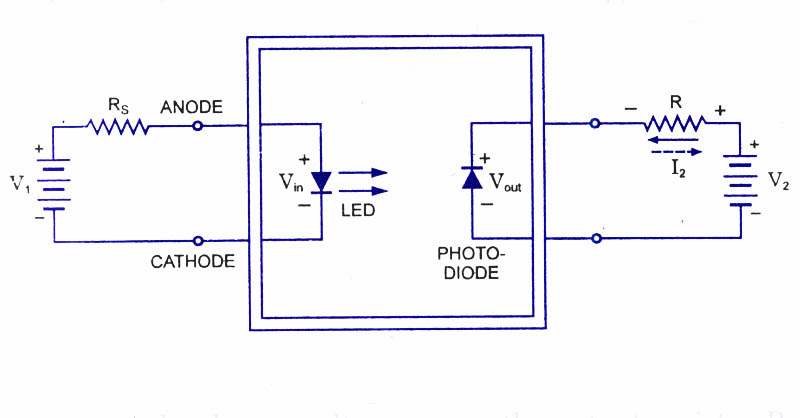
\includegraphics[width=.8\linewidth]{04/01_optocoupler_scheme.jpg}
  \caption{Schema optocuplor \cite{OptocouplerCircuitsToday}}
  \label{fig:sub1}
\end{subfigure}%
\begin{subfigure}{.5\textwidth}
  \centering
  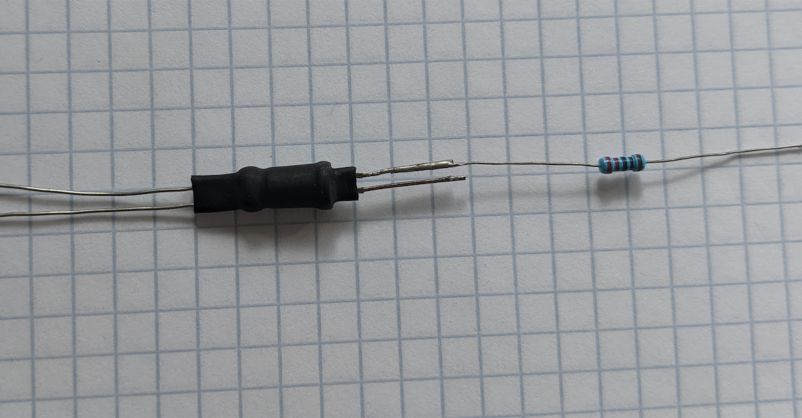
\includegraphics[width=.8\linewidth]{04/02_optocoupler_assembly.png}
  \caption{Ansanblu realizat manual}
  \label{fig:sub2}
\end{subfigure}
\caption{Schema electrica optocuplor (a) si rezultat ansablu (b)}
\label{fig:test}
\end{figure}

Deoarece aveam nevoie sa scurtcircuitez un contactor pe partea terminalului \acrshort{pots} am omis rezistenta legata fotorezistorului. Atunci cand ledul este aprins, rezistenta fotorezistorului scade, comportandu-se aproape ca un conductor ideal, atingand lamelele contactorului corespunzator receptorului.

\subsection {Webserver NodeJS}

NodeJS este un

\subsubsection {NestJS}

Metadate si chestii, dependency injection si MVC la aplicatie

\subsubsection {Mutex}

Din natura asincrona a limbajului si posibilitatea sistemului de a avea mai mult de un utilizator, trebuie luat in considerare cazul in care mai multi utilizatori incearca sa interactioneze cu sistemul in acelasi timp. Asadar, trebuie implementat un mecanism similar semaforului binar, numit mutex. Diferenta dintre acestea fiind ca in cazul mutexului, doar detinatorul original poate sa il elibereze spre a fi folosit.

Acest comportament este de dorit pentru a informa clientii serviciului in cazul in care requestul nu poate fi satisfacut deoarece resursa este ocupata de altcineva.

\begin{figure}[h!]
  \centering
  \fbox {
    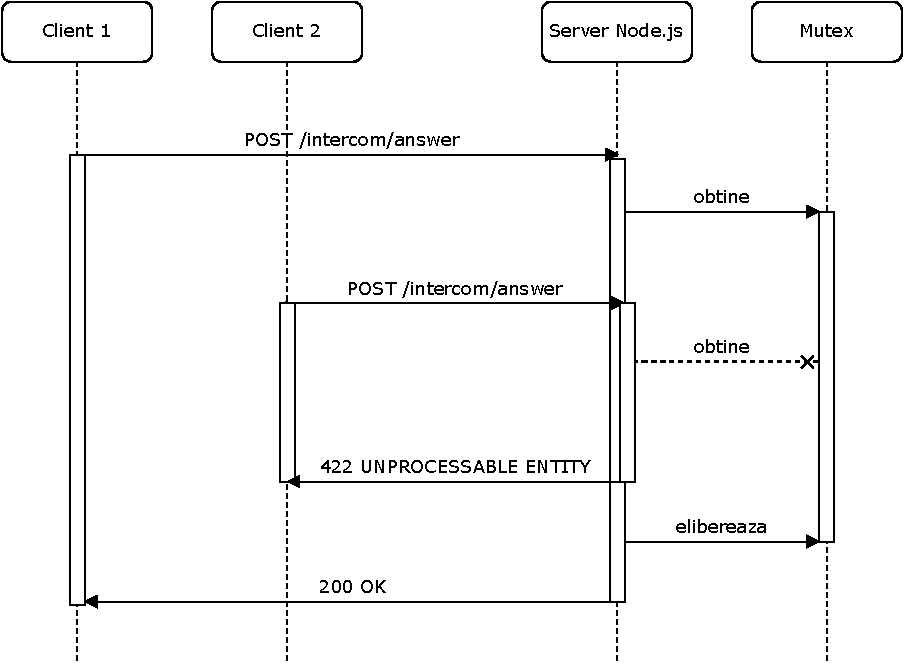
\includegraphics[width=0.6\textwidth]{04/03_mutex_diagram.pdf}  
  }
  \caption{Ilustrare resursa disputata intre doi utilizatori}
\end{figure}


\subsubsection {Validare}

Foloseste functii din Typescript si NestJS pentru a adauga si citi metadate prin intermediul decoratorilor de metode.

\subsubsection {Autentificare}

La fel ca mai sus

\subsubsection {Roluri}

Din nou decorator


\subsection {Android}

Android este o platforma mobile care s-a maturizat pe parcusul a 12 versiuni majore si principalul competitor de piata al iOS.


\section {Implementarea sistemului}


\section {Testarea sistemului}